\documentclass[12pt]{article}

\usepackage[spanish,es-tabla]{babel}
\usepackage[utf8]{inputenc}
\usepackage{lipsum}
\usepackage{graphicx}
\usepackage[none]{hyphenat}
\usepackage{biblatex}
\usepackage{csquotes}
\usepackage{hyperref}
\usepackage[raggedright]{titlesec}
\usepackage{amsmath}
\usepackage[a4paper,top=3.5cm,bottom=3.5cm,left=3cm,right=3cm,marginparwidth=1.5cm]{geometry}
\usepackage{multirow}
\usepackage{array}
\usepackage{tabularx}
\usepackage[small]{caption}
\usepackage{flafter} 
\usepackage{subfig} 

\usepackage{algorithm}
\usepackage{algpseudocode}

% ALGORITMOS EN ESPAÑOL
\makeatletter
    \renewcommand{\ALG@name}{Algoritmo}
    \renewcommand{\listalgorithmname}{
    Índice de \ALG@name s}
\makeatother

% AUMENTAR PADDING A FILAS
\setlength\extrarowheight{4pt}

% ESTABLECER DIRECTORIO DE FIGURAS Y BIBLIOGRAFIA
\graphicspath{ {./Figuras} } 
\addbibresource{Otros/bibliografia.bib}

% ESPACIOS TITULOS
\titlespacing*{\section}
{0pt}{5.5ex plus 1ex minus .2ex}{4.3ex plus .2ex}
\titlespacing*{\subsection}
{0pt}{5.5ex plus 1ex minus .2ex}{4.3ex plus .2ex}
\titlespacing*{\subsubsection}
{0pt}{5.5ex plus 1ex minus .2ex}{4.3ex plus .2ex}

% NUEVO TIPO DE COLUMNA CENTRADO
\newcolumntype{Y}{>{\centering\arraybackslash}X}

% QUITAR INDENTACION
\setlength{\parindent}{0pt}

% FORMTO PORTADA
\makeatletter
\renewcommand{\maketitle}{
\begin{center}

\pagestyle{empty}
\phantom{.}
\vspace{0cm}

{\Huge \bf \@title\par}
\vspace{2.5cm}

{\LARGE Roberto Juárez Bote}\\[1cm]

{\Large\@date}

\vfill

\includegraphics[scale=0.3]{logo.png}
\vfill

{Tutor\\[0.2cm]\Large Jesús S. Aguilar Ruiz}\\[0.4cm]Código del TFG\\[0.2cm]{\Large 20-21-C1}\\[2cm]
Trabajo Final de Grado\\
Universidad Pablo de Olavide

\end{center}
\thispagestyle{empty}
\clearpage
}
\makeatother

\begin{document}
    \sloppy 
    % TITULO
    \title{\textbf{EVALUACIÓN DE MODELOS PREDICTIVOS}}
    \date{\today}
    \maketitle

    % INDICES
    \thispagestyle{empty}
    \tableofcontents
    \clearpage
    \thispagestyle{empty}
    \listoffigures
    \clearpage
    \thispagestyle{empty}
    \listoftables
    \clearpage
    \thispagestyle{empty}
    \listofalgorithms
    \clearpage

    % OTRAS SECCIONES
    \thispagestyle{empty}
\section*{Lista de Acrónimos}

TP: \textit{True Positive} (Verdadero Positivo)
\medbreak
TN: \textit{True Negative} (Verdadero Negativo)
\medbreak
FP: \textit{False Positive} (Falso Positivo)
\medbreak
FN: \textit{False Negative} (Falso Negativo)
\medbreak
ACC: \textit{Accuracy} (Exactitud)
\medbreak
TPR: \textit{True Positive Rate} (Sensibilidad)
\medbreak
TNR: \textit{True Negative Rate} (Especificidad)
\medbreak
LR: \textit{Likehood Ratio} (Razón de Verosimilitud)
\medbreak
LR+: \textit{Positive Likehood Ratio} (Razón de Verosimilitud Positiva)
\medbreak
LR-: \textit{Negative Likehood Ratio} (Razón de Verosimilitud Negativa)
\medbreak
DOR: \textit{Diagnostic Odds Ratio}
\medbreak
YI: \textit{Youden's Index} (Índice de Youden)
\medbreak
MCC: \textit{Matthews Correlation Coefficient} (Coeficiente de Correlación de Matthews)
\medbreak
DP: \textit{Discriminant Power} (Poder Discriminante)
\medbreak
F$_{1}$: \textit{F-score} (Medida F)
\medbreak
MK: \textit{Markedness}
\medbreak
BCR: \textit{Balanced Accuracy} (Exactitud Balanceada)
\medbreak
GM: \textit{Geometric Mean} (Media Geométrica)
\medbreak
OP: \textit{Optimization Precision} (Precisión de Optimización)
\medbreak
ROC: \textit{Receiver Operating Characteristic}
\medbreak
PR: \textit{Precision Recall}
\medbreak
AUAC: \textit{Area Under A-Curve}


\clearpage
    \thispagestyle{empty}
\section*{Resumen}

En este documento se hace una revisión de los métodos más representativos que existen en la actualidad para la evaluación de modelos predictivos.
También se introduce el concepto de curva-A, un nuevo gráfico que parte de la fórmula de validación descrita por Brier en el artículo \textit{Verification of Forecasts Expressed in Terms of Probability} \cite{brie_1950} publicado en 1950. La curva-A ofrece una nueva forma de representación gráfica que permite evaluar la calidad predictiva de un modelo, este nuevo método se puede aplicar tanto a modelos de clasificación binaria cómo a modelos de clasificación multi etiqueta. En este documento además se incluye un estudio comparativo entre la curva ROC y la curva-A, el objetivo del estudio es ofrecer una visión general de cada una de las curvas cubriendo aspectos como la definición, el funcionamiento, las propiedades, etc. El estudio en última instancia busca presentar una comparativa entre las dos curvas analizando las ventajas e inconvenientes que ofrece la curva-A.

\bigbreak

En el apartado técnico se ha realizado una implementación en KNIME de cada uno de los métodos que se presentan en este documento. Adicionalmente, se ha elaborado un flujo de trabajo que permite ejecutar el proceso completo de entrenamiento y evaluación de forma automática para varios ficheros de datos. El proceso también incluye una vista en la que se presenta un informe con los resultados obtenidos utilizando cada fichero de datos. Finalmente, se incluyen varios casos prácticos en los que se realiza un estudio para distintos modelos predictivos a partir de los métodos de evaluación implementados.

\clearpage

    % CONTENIDO
    \setcounter{page}{1}
    \section{Introducción}

El proyecto consiste en el estudio de las principales técnicas tanto analíticas como gráficas que se utilizan en la actualidad para la evaluación de modelos predictivos. A continuación, se describen los principales objetivos del proyecto:

\bigbreak

\begin{itemize}
    \item Introducir y dar a conocer las propiedades y usos de la curva-A. El objetivo es sentar una base sólida para la aplicación de este nuevo método.
    \item Presentar una selección de los métodos más usados para la evaluación de modelos predictivos. Estos métodos han sido ampliamente documentados en estudios anteriores, en este documento se propone una revisión de los más destacados.
    \item Realizar un estudio comparativo entre los diferentes métodos gráficos que ayude a determinar cuáles son las ventajas e inconvenientes de la aplicación de la curva-A. 
    \item Elaborar una experimentación que permita aplicar los métodos de evaluación a diferentes casos prácticos. Cada caso práctico cuenta con un conjunto de datos asociado, los conjuntos de datos cubren diferentes tipos de modelos predictivos.
\end{itemize}

\bigbreak

El contenido del proyecto se divide en dos grandes bloques. En el primer bloque se realiza un estudio teórico en el que se incluye la revisión de los diferentes métodos de evaluación. El segundo bloque cubre la parte experimental del proyecto, en este bloque se recopilan e interpretan los resultados obtenidos para los diferentes casos prácticos.

\clearpage
    \section{Técnicas para la Evaluación de Modelos Predictivos}

%En este punto, se puede hablar de conjunto de test, train etc

En este apartado se realiza una revisión de los principales métodos


Los modelos predictivos en los que se centra esta sección son modelos de clasificación en los que se tiene un número discreto de posibles valores para la clase objetivo, por ejemplo, un conjunto de datos con registros de emails, con una clase que marca cada registro como spam o no spam. El modelo predictivo en este caso está entrenado para predecir un valor u otro de esta clase en función del resto de atributos. En esta sección se ofrece un análisis de las diferentes técnicas tanto analíticas como gráficas para la evaluación de modelos predictivos.

\subsection{Matriz de confusión}

La matriz de confusión es una herramienta que se suele aplicar en las primeras fases del análisis, permite organizar los indicadores de rendimiento obtenidos para un modelo predictivo, en general, ofrece un recuento de los registros en base a la clase real de cada registro y a la predicción que realiza el modelo. La matriz de confusión se define como una matriz cuadrada de $NxN$ elementos donde $N$ es el numero de clases presentes en el modelo, cada fila de la matriz de confusión define la clase real del registro y cada columna define la clase predicha por el modelo o viceversa.

\bigbreak

En la matriz de confusión se definen cuatro indicadores, estos indicadores ofrecen una visión general del rendimiento del modelo y son la base para el calculo de algunas métricas mas avanzadas que se tratan en secciones posteriores de este documento. Los indicadores definidos en la matriz de confusión son:

\begin{itemize}
    \item Verdadero Positivo: Registros de clase real positiva y en los que la predicción se hace correctamente.
    \item Verdadero Negativo: Registros de clase real negativa y en los que la predicción se hace correctamente.
    \item Falso Negativo: Registros de clase real positiva y en los que la predicción se hace incorrectamente.
    \item Falso Positivo: Registros de clase real negativa y en los que la predicción se hace incorrectamente.
\end{itemize}

\pagebreak

La matriz de confusión se define de forma general para modelos de clasificación multi-etiqueta, sin embargo, a la hora de obtener los indicadores de rendimiento para modelos de clasificación con mas de dos clases tenemos que definir $N$ matrices una por cada clase del modelo, en cada matriz se define positiva una de las clases y se agrupan como negativas el resto, de esta forma, el estudio que se realiza a partir de las diferentes sub-matrices ya no es un estudio global, sino que es especifico para cada clase concreta.

\begin{table}[ht]
    \centering
    \begin{tabular}[t]{ccc}
                 & Positivo*          & Negativo*          \\\hline
        Positivo & Verdadero Positivo & Falso Negativo     \\\hline
        Negativo & Falso Positivo     & Verdadero Negativo \\\hline
    \end{tabular}

    \caption{Matriz de confusión 2x2.}
    \label{tab:1}
\end{table}

%%%%%%%%%%%%%%%%%%%%%%%%%%%%%%%%%%%%%%%%%%%%%%%%%%%%%%%%% SUBSECCION METODOS ESTADISTICOS

\subsection{Métodos estadísticos}

%%%%%%%%%%%%%%%%%%%%%%%%%%%%% SUBSUBSECCION Exactitud

\subsubsection{Exactitud}

La exactitud es una de las medidas más utilizadas a la hora de establecer la calidad general de un modelo predictivo. Este método representa la tasa de acierto que se obtiene al aplicar un modelo predictivo sobre un conjunto de \textit{test}. El calculo de esta medida se hace en base a los cuatro indicadores de rendimiento definidos en la matriz de confusión. El resultado que ofrece se encuentra en el intervalo de cero a uno, los valores próximos a cero corresponden a modelos con una baja tasa de acierto, mientras que los valores próximos a uno corresponden a modelos con una alta tasa de acierto. En términos generales los modelos que obtienen un resultado inferior a media unidad son poco prometedores, en promedio tienen una tasa de aciertos inferior a la de un modelo de clasificación aleatoria. Por último, cabe destacar que es un método independiente del número de clases, se puede aplicar tanto a modelos de clasificación binaria como a modelos de clasificación multi-etiqueta.

\bigbreak

\begin{equation}\tag*{}
    ACC = \frac{TP+TN}{TP+TN+FP+FN}
\end{equation}

%%%%%%%%%%%%%%%%%%%%%%%%%%%%% SUBSUBSECCION SENSIBILIDAD Y ESPECIFICIDAD

\subsubsection{Sensibilidad y Especificidad}

La sensibilidad y la especificidad son dos medidas complementarias que ofrecen una representación por separado de la exactitud del modelo. En primer lugar, la sensibilidad es un método que mide la tasa de acierto del modelo sobre instancias de clase positiva. De igual forma, la especificidad mide la tasa de acierto del modelo únicamente sobre instancias de clase negativa. En ambos casos el calculo se hace a partir de los indicadores de rendimiento definidos en la matriz de confusión. El resultado obtenido se encuentra en el intervalo de cero a uno, los valores próximos a cero indican una baja tasa de acierto, mientras que los valores próximos a uno indican una alta tasa de acierto. A diferencia de la exactitud estas dos medidas son sensibles al numero de clases del modelo, solo se pueden aplicar a modelos de clasificación binaria. Para su aplicación a modelos de clasificación multi-etiqueta se puede aplicar el método a una clase concreta que definimos como positiva, el resto de clases se agrupan como clase negativa.

\bigbreak
\begin{equation}\tag*{}
    TPR = \frac{TP}{P} = \frac{TP}{TP+FN}
    \hspace{1cm}
    TPN = \frac{TN}{N} = \frac{TN}{TN+FP}
\end{equation}


%%%%%%%%%%%%%%%%%%%%%%%%%%%%% SUBSUBSECCION PRECISION Y PRECISION INVERSA

\subsubsection{Precisión y Precisión Inversa}

\bigbreak
\begin{equation}\tag*{}
    TPR = \frac{TP}{P} = \frac{TP}{TP+FN}
    \hspace{1cm}
    TPN = \frac{TN}{N} = \frac{TN}{TN+FP}
\end{equation}

%%%%%%%%%%%%%%%%%%%%%%%%%%%%% SUBSUBSECCION RAZON DE VEROSIMILITUD

\subsubsection{Ratios de Probabilidad}

Los ratios de probabilidad son métodos que se utilizan fundamentalmente en el ámbito medico para la evaluación de pruebas diagnosticas, en general miden como varia la probabilidad de padecer una determinada patología en función de si el paciente presenta un determinado estado o no lo presenta, de forma similar, para el ámbito de la evaluación de modelos predictivos los ratios de probabilidad nos informan de como varia la probabilidad de que un registro sea positivo en función de la predicción que se realiza.
\bigbreak
Tenemos dos tipos de ratios de probabilidad, el ratio de probabilidad positivo LR+ y el ratio de probabilidad negativo LR-. El ratio de probabilidad positivo mide como varia la probabilidad de que un registro sea positivo cuando se clasifica como positivo, así mismo, el ratio de probabilidad negativo mide como varia la probabilidad de que un registro sea positivo cuando se clasifica como negativo, en ambos casos el calculo de las métricas se hace a partir de la sensibilidad y la especificidad. Es importante destacar que los ratios de probabilidad no guardan una relación de proporcionalidad, el cambio en la probabilidad de que un registro sea de clase positiva no varia en la misma proporción cuando el registro se clasifica como positivo que cuando se clasifica como negativo.

\bigbreak
El ratio de probabilidad positivo es una medida que toma valores mayores que la unidad,  ofrece un mejor indicador cuanto mayor sea el valor que toma, por el contrario el ratio de probabilidad negativo se encuentra en el rango de valores $[0, 1]$, ofrece un mejor indicador cuanto mas próximo al cero se encuentre, en ambos casos los valores próximos a la unidad no ofrecen resultados concluyentes. En la Tabla \ref{tab:2} podemos ver una aproximación de la variación en la probabilidad que se produce para diferentes valores.
\bigbreak

\begin{table}[ht]
    \centering
    \begin{tabular}[t]{ccc}
        Variación en la probabilidad (\%) & \hspace{20pt}LR+\hspace{20pt} & LR- \\\hline
        +45                              & 10                            & -   \\\hline
        +30                              & 5                             & -   \\\hline
        +15                              & 2                             & -   \\\hline
        0                                & 1                             & 1   \\\hline
        -15                              & -                             & 0.5 \\\hline
        -30                              & -                             & 0.2 \\\hline
        -45                              & -                             & 0.1 \\\hline
    \end{tabular}
    \caption{Variación en la probabilidad para diferentes ratios de probabilidad.}
    \label{tab:2}
\end{table}

Para el calculo de estas dos métricas se utilizan

\bigbreak
\begin{equation}\tag*{}
    LR^{\phantom{.}+}    = \frac{TPR}{1-TNR}
    \hspace{1cm}
    LR^{\phantom{.}-} = \frac{1-TPR}{TNR}
\end{equation}
\bigbreak

\begin{table}[ht]
    \centering
    \begin{tabular}[t]{lcc}
            & \hspace{20pt}Normal\hspace{20pt} & Tumoral \\\hline
        TPR & 0.667                            & 0.833   \\\hline
        TNR & 0.833                            & 0.667   \\\hline
        LR+ & 4.000                            & 2.500   \\\hline
        LR- & 0.400                            & 0.250   \\\hline
    \end{tabular}
    \caption{Métricas obtenidas a partir del fichero de datos breast\_gse26910.}
    \label{tab:3}
\end{table}



    \section{Curva A}

En este punto se presenta una nueva herramienta gráfica que permite la evaluación de un modelo predictivo en base al error que se comente en la predicción. Este nuevo método surge de la necesidad de obtener una forma de representación gráfica que se pueda aplicar tanto a modelos de clasificación binaria como a modelos de clasificación multi etiqueta. La representación gráfica del error se obtiene a partir la fórmula de verificación propuesta por Brier en el artículo \textit{Verification of Forecasts Expressed in Terms of Probability} \cite{brie_1950}.

\bigbreak

La fórmula de verificación de Brier se define como el sumatorio del error cuadrático medio entre la clase y las diferentes probabilidades que asigna el modelo a cada etiqueta. La fórmula de verificación constituye un punto de partida ideal ya que se define teniendo en cuenta su aplicación a modelos de clasificación con más de dos clases. La representación del error que se hace en la fórmula de verificación también es independiente del balance entre el número de instancias de cada clase, esto supone un punto positivo a tener en cuenta.

\bigbreak

\begin{equation}
    P = \frac{1}{n}\sum_{j=1}^{r}\sum_{i=1}^{n}{(f_{ij}-E_{ij})^{2}}
    \label{eq:BrierScore}
\end{equation}

\bigbreak


En la ecuación \ref{eq:BrierScore} se representa la definición original de la fórmula de verificación. El parámetro $E_{ij}$ indica si la clase del registro $i$ coincide con la etiqueta $j$. El indicador $f_{ij}$ representa la probabilidad que se le asigna al registro $i$ de pertenecer a la clase $j$.

\bigbreak

El resultado que se obtiene al aplicar la fórmula de verificación se encuentra en el intervalo de cero a dos. En el caso de un modelo de clasificación binario en el que se predicen positivos los registros negativos y negativos los registros positivos, el resultado obtenido es de dos unidades. Por el contrario, si se clasifican correctamente todos los registros, el resultado obtenido es de cero.

\bigbreak

Para facilitar la interpretación de la curva A, se propone una modificación de la fórmula de verificación. El objetivo de redefinir la fórmula es obtener una gráfica que tenga una interpretación similar a la curva ROC. En la ecuación \ref{eq:A} aparece representada la fórmula que se utilizara en el cálculo de la curva A. El resultado que se obtiene de la nueva fórmula se encuentra en el intervalo de cero a uno, los valores próximos a uno indican tasas de error más bajas, mientras que los valores próximos a cero indican tasas de error más altas. Hay que tener en cuenta que la aplicación del método ya no se hace sobre todas las instancias del modelo, sino que se aplica de forma individual a cada registro.

\bigbreak

\begin{equation}
    A = 1-\frac{\sum_{i=1}^{r}{(f_{i}-E_{i})^{2}}}{2}
    \label{eq:A}
\end{equation}

\bigbreak



La representación de la curva A se hace a partir de los valores obtenidos al aplicar la formula \ref{eq:A} a cada uno de los registros del conjunto de entrenamiento. Es importante aclarar que antes de generar la curva el conjunto de datos con los resultados tiene que estar ordenado. Para representar los puntos en la gráfica, a cada resultado se le asigna un valor equidistante entre cero y uno que permite representar los resultados obtenidos en base al orden establecido. En el eje de ordenadas se representan los resultados obtenidos al aplicar la formula, en el eje de abscisas se representan los puntos de apoyo calculados para cada resultado.

\bigbreak

La interpretación que se hace de la gráfica es muy similar a la que se hace en la curva ROC, cuanto más se aproxime la gráfica al punto $(0, 1)$ mejores tasas de acierto tendrá el modelo. Las curvas que se encuentren por debajo de la diagonal secundaria indican que el modelo tiene tasas de acierto inferior a las de un modelo de clasificación aleatoria. En la Figura \ref{fig:1} se puede ver en azul la curva que presenta un modelo con una clasificación perfecta, por otro lado, la curva naranja es la curva que presenta un modelo de clasificación aleatoria.

\bigbreak

\begin{figure}[htp]
    \centering
    \includegraphics[scale=0.45]{interpretación_curva_a.PNG}
    \caption{Gráfica para la interpretación de la curva A.}
    \label{fig:1}
\end{figure}

\bigbreak

En la Figura \ref{fig:2} se muestra una comparativa entre las curvas A y ROC obtenidas para un modelo de clasificación con cuatro etiquetas. En el primer gráfico se puede observar que la aplicación de la curva ROC en un modelo con cuatro etiquetas implica un aumento de la complejidad en la interpretación de los resultados. El uso de curvas ROC en modelos de clasificación multi etiqueta, también afecta a las conclusiones que se pueden extraer de la calidad general del modelo, esta incapacidad de sacar conclusiones afecta negativamente al proceso de toma de decisiones. La curva A supone una excelente alternativa, el gráfico que se genera para un modelo de clasificación con cuatro etiquetas está compuesto tan solo por una curva, esto supone una mejora en la claridad y en la interpretación de la información. 

\bigbreak

\begin{figure}[htp]
    \centering
     \subfloat[Curva ROC]{
       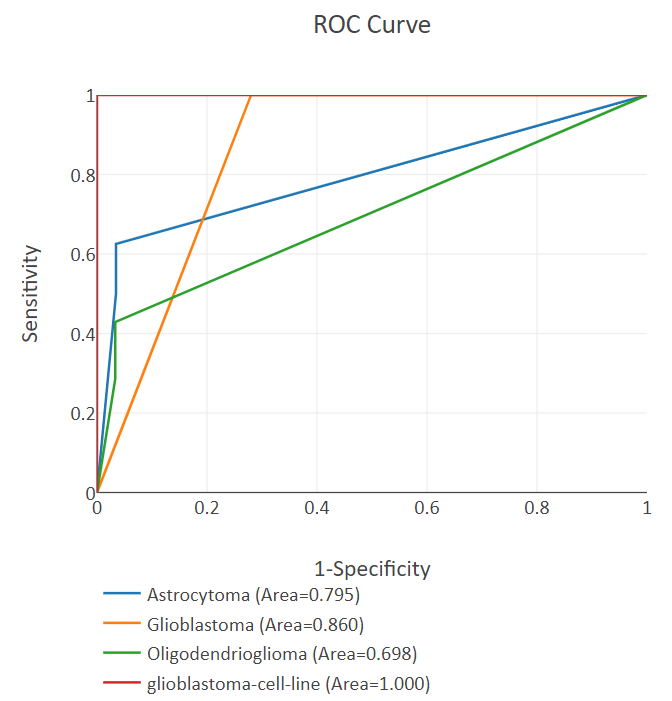
\includegraphics[width=0.45\textwidth]{brain_gse15824_ROC.PNG}}
     \subfloat[Curva A]{
       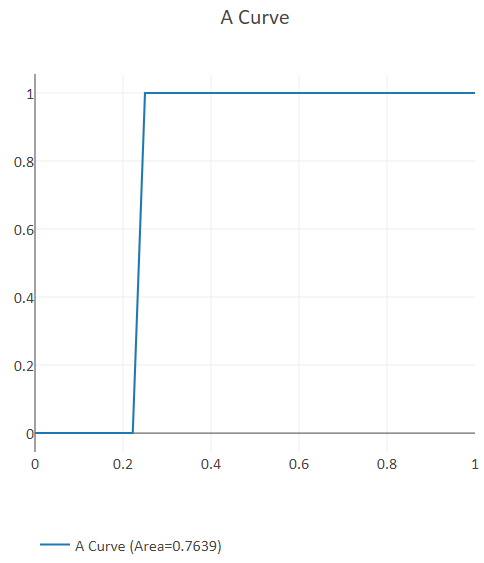
\includegraphics[width=0.45\textwidth]{brain_gse15824_A_CURVE.PNG}}
    \caption{Curvas obtenidas para el fichero brain\_gse15824.csv.}
    \label{fig:2}
\end{figure}

\bigbreak

Hay situaciones en las que no es posible establecer una comparativa exclusivamente gráfica entre varias representaciones de la curva A. La definición que se hace de la curva implica que el área bajo la curva aumenta a medida que la curva se aproxima al punto (0, 1), es decir, cuanto mayor es el valor del área bajo la curva mejores tasas de acierto obtiene el modelo. El área bajo la curva, también se puede considerar como un indicador de la calidad general del modelo. El resultado que ofrece, se encuentra en el intervalo de cero a uno, los valores cercanos a uno indican que el modelo tiene buenas tasas de acierto en la predicción, mientras que los valores próximos a cero indican la presencia de un modelo con una muy baja capacidad predictiva. Por último, cabe destacar el grado de similitud entre la exactitud y el área bajo la curva A, esta relección será objeto de estudio en la parte experimental.

\bigbreak

El Algoritmo \ref{al:a_curve} presenta una implementación para obtener los puntos que definen la curva-A, la función recibe como entrada dos matrices de datos. En la variable L se define una matriz de dimensión $NxM$ donde $N$ es el número de registros y $M$ es el número de etiquetas, en cada celda de la matriz se indica con los valores cero o uno si el registro $i$ tiene asignada la etiqueta $j$. En la variable P se define una matriz de dimensión $NxM$ donde $N$ es el número de registros y $M$ es el número de etiquetas, en cada celda se almacena la probabilidad que asigna el modelo al registro $i$ de pertenecer a la clase $j$. La complejidad del algoritmo es $\mathcal{O}(n \cdot m + n \log(n))$, sin embargo, el número de etiquetas se puede considerar como un valor constante dentro del problema al aplicar esta simplificación la complejidad pasa a ser igual al coste de ordenación $\mathcal{O}(n \log(n))$. El algoritmo recorre los distintos registros (bucle, línea 4), por cada registro aplica la formula \ref{eq:A}. Para la aplicación de la formula se calcula en primer lugar el valor del sumatorio, una vez calculado se divide el resultado entre dos y se le resta a la unidad. Por ultimo, se ordena el conjunto de datos R siguiendo un orden ascendente (función, línea 11).

\bigbreak


\bigbreak

\begin{algorithm}
    \caption{Curva-A}
        \begin{algorithmic}[1]
            \State $L$
            \State $P$
            \State $R = [\phantom{.}]$

            \For{$i = 1$ to $|L|$}
                \State $R[i] = 0$
                \For{$j = 1$ to $|L[i]|$}
                    \State $R[i]$ += pow $(L[i][j]-P[i][j], 2)$
                \EndFor
                \State $R[i] = 1 - (R[i]/2)$
            \EndFor
            \State  sort $(R, asc)$
    \end{algorithmic}
    \label{al:a_curve}
\end{algorithm}

\bigbreak

\begin{table}[htp]
    \small
    \centering
    \begin{tabular}{c c c c c c c c c}
        ID  & \hspace{10pt}$L_{0}$  & \hspace{10pt}$L_{1}$  & \hspace{10pt}$L_{2}$  & \hspace{10pt}$P_{0}$ & \hspace{10pt}$P_{1}$ & \hspace{10pt}$P_{2}$  & \hspace{10pt}$E_{R}$ & \hspace{10pt}$1-E_{R}/2$ \\\hline
        $1$ & \hspace{10pt}$1$ & \hspace{10pt}$0$ & \hspace{10pt}$0$ & \hspace{10pt}$0.5$ & \hspace{10pt}$0.2$ & \hspace{10pt}$0$ & \hspace{10pt}$0.29$ & \hspace{10pt}$0.855$           \\\hline
        $2$ & \hspace{10pt}$0$      & \hspace{10pt}$1$ & \hspace{10pt}$0$   & \hspace{10pt}$0.1$    & \hspace{10pt}$0.8$ & \hspace{10pt}$0.1$ & \hspace{10pt}$0.06$ & \hspace{10pt}$0.97$     \\\hline
        $3$ & \hspace{10pt}$1$      & \hspace{10pt}$0$ & \hspace{10pt}$0$   & \hspace{10pt}$1$    & \hspace{10pt}$0$ & \hspace{10pt}$0$ & \hspace{10pt}$0$  & \hspace{10pt}$1$   \\\hline
        $4$ & \hspace{10pt}$0$      & \hspace{10pt}$0$  & \hspace{10pt}$1$  & \hspace{10pt}$0$    & \hspace{10pt}$0.3$ & \hspace{10pt}$0.7$ & \hspace{10pt}$0.18$  & \hspace{10pt}$0.91$    \\\hline
        $5$ & \hspace{10pt}$0$      & \hspace{10pt}$1$ & \hspace{10pt}$0$   & \hspace{10pt}$1$    & \hspace{10pt}$0$ & \hspace{10pt}$0$ & \hspace{10pt}$2$  & \hspace{10pt}$0$    \\\hline
        $6$ & \hspace{10pt}$0$      & \hspace{10pt}$0$  & \hspace{10pt}$1$  & \hspace{10pt}$0$    & \hspace{10pt}$0$ & \hspace{10pt}$1$ & \hspace{10pt}$0$ & \hspace{10pt}$1$    \\\hline
    \end{tabular}
    \caption{Ejemplo propuesto para el calculo de los puntos que representan la curva-A.}
    \label{tab:5}
\end{table}

\clearpage
    \section{Tecnologías}

En esta sección se cubren las diferentes tecnologías que se han utilizado para el desarrollo de este trabajo final de grado, también se detalla el uso que se le ha dado a cada una de las herramientas. 

\bigbreak

En primer lugar, Knime es una potente herramienta de código abierto orientada al análisis de datos, es ideal para proyectos relacionados con minería de datos, inteligencia artificial, etc. Knime es la herramienta principal con la que se ha desarrollado la parte experimental del proyecto, el objetivo principal para uso de Knime es ofrecer una implementación de los diferentes métodos y gráficas que se han ido desarrollando a lo largo del documento. En este sentido, se realiza un flujo de trabajo completo en el que se incluyen las fases de carga de datos, de generación del modelo predictivo, de evaluación del modelo y finalmente de reporte de resultados. Cabe destacar que se han utilizado algunas extensiones que aumentan la funcionalidad de la herramienta, como es el caso de la extensión para la integración de Python o la extensión para la generación de datos. A continuación, se enumeran algunas de las principales ventajas que ofrece Knime:

\begin{itemize}
    \item Permite la creación de un flujo de trabajo que incluye las principales fases que componen un proyecto de análisis de datos. 
    \item Knime ofrece una interfaz visual e intuitiva que permite a través del uso de nodos la visualización de datos, la creación de modelos predictivos, la generación de reportes, etc.
    \item Es una herramienta de código abierto.
    \item Permite la integración con lenguajes de programación como Java, Python, R, etc. Esto aporta un extra de flexibilidad a la hora de hacer ciertas operaciones o utilizar librerías propias de un lenguaje especifico.
    \item La aplicación de escritorio está disponible para sistemas operativos Windows, MacOs y Linux.
\end{itemize}

\bigbreak

Otra de las aplicaciones que más utilizadas a lo largo del desarrollo ha sido Git. Git es un sistema de control de versiones distribuido, permite mantener un control sobre el desarrollo que se ha realizado. Git junto con Github me han permitido tener una copia de seguridad actualizada en la nube, también me han habilitado la posibilidad de desarrollar el proyecto desde varios equipos de forma sencilla.

\clearpage
    \section{Experimentación}

\subsection{Descripción de la Experimentación}

En esta sección se cubre la parte experimental del proyecto. Todo el desarrollo ha sido realizado utilizando Knime, una herramienta para el análisis de datos ampliamente utilizada en este sector. El objetivo principal es ofrecer una comparación entre las diferentes métricas vistas en secciones anteriores, poniendo especial énfasis en la comparación de estas con el nuevo método grafico curva-A.

\bigbreak

Para la experimentación vamos a partir de una selección de seis ficheros de datos, todos los ficheros utilizados en la experimentación han sido obtenidos de la web del SBCB \url{https://sbcb.inf.ufrgs.br/cumida}, en general los conjuntos de datos forman parte de un repositorio de datos relacionado con diversos tipos de cáncer, estos conjuntos de datos cubren un amplio rango de casuísticas y suponen una excelente elección para entrenar modelos tanto de clasificación binaria como modelos de clasificación multi etiqueta.

\bigbreak

El escenario de pruebas que se ha definido no se realiza ningún tipo de preprocesado al conjunto de datos de entrada, únicamente se aplica una normalización, ya que supone una mejora en el rendimiento de los modelos basados en el teorema de Bayes. Para los diferentes conjuntos de datos, se va a aplicar un predictor basado en el teorema de Bayes. Para la validación aplicamos validación cruzada con 10 iteraciones, el uso de este tipo de validación está muy extendido en proyectos de análisis de datos, ya que ofrece en general grandes resultados. Para cada fichero presentaremos los resultados obtenidos fruto de aplicar las métricas vistas anteriormente al conjunto de datos correspondiente. Posteriormente se exponen las conclusiones.


\clearpage

\subsection{Resultados de la Experimentación}


%%%%%%%%%%%%%%%%%%%%%%%%%%%%%%%%%%%%%%%%%%%%%%%%%%%%%%% RESULTADO
\subsubsection{Fichero brain\_gse15824.csv}

\begin{table}[htp]
    \small
    \centering
    \begin{tabularx}{\columnwidth}{Y Y}
        ACC       & AUAC    \\\hline
        $0.757$   & $0.764$ \\\hline
    \end{tabularx}
    \caption{Resultados globales para el fichero brain\_gse15824.csv.}
    \label{tab:10}
\end{table}

\begin{table}[htp]
    \small
    \centering
    \begin{tabularx}{\columnwidth}{l c c c c}
                &  Astrocytoma  & Glioblastoma & Oligodendrioglioma   & Glioblastoma-cell-line   \\\hline
        TPR     &  $0.500$      & $1.000$      & $0.286$              & $1.000$                  \\\hline
        TNR     &  $0.966$      & $0.720$      & $0.967$              & $1.000$                  \\\hline
        PPV     &  $0.800$      & $0.632$      & $0.667$              & $1.000$                  \\\hline
        NPV     &  $0.875$      & $1.000$      & $0.853$              & $1.000$                  \\\hline
        LR+     &  $14.500$     & $3.571$      & $8.571$              & -                        \\\hline
        LR-     &  $0.518$      & $0.000$      & $0.739$              & $0.000$                  \\\hline
        DOR     &  $28.000$     & -            & $11.600$             & -                        \\\hline
        YI      &  $0.466$      & $0.720$      & $0.252$              & $1.000$                  \\\hline
        MCC     &  $0.561$      & $0.674$      & $0.362$              & $1.000$                  \\\hline
        DP      &  $0.798$      & -            & $0.587$              & -                        \\\hline
        $F_{1}$ &  $0.615$      & $0.774$      & $0.400$              & $1.000$                  \\\hline
        MK      &  $0.675$      & $0.632$      & $0.520$              & $1.000$                  \\\hline
        BCR     &  $0.733$      & $0.860$      & $0.626$              & $1.000$                  \\\hline
        GM      &  $0.695$      & $0.849$      & $0.526$              & $1.000$                  \\\hline
        OP      &  $0.547$      & $0.648$      & $0.294$              & $1.000$                  \\\hline
        Jaccard &  $0.444$      & $0.632$      & $0.250$              & $1.000$                  \\\hline

    \end{tabularx}
    \caption{Resultados agrupados por clase para el fichero brain\_gse15824.csv.}
    \label{tab:11}
\end{table}

\bigbreak

\begin{figure}[htp]
    \centering
     \subfloat[Curva ROC]{
       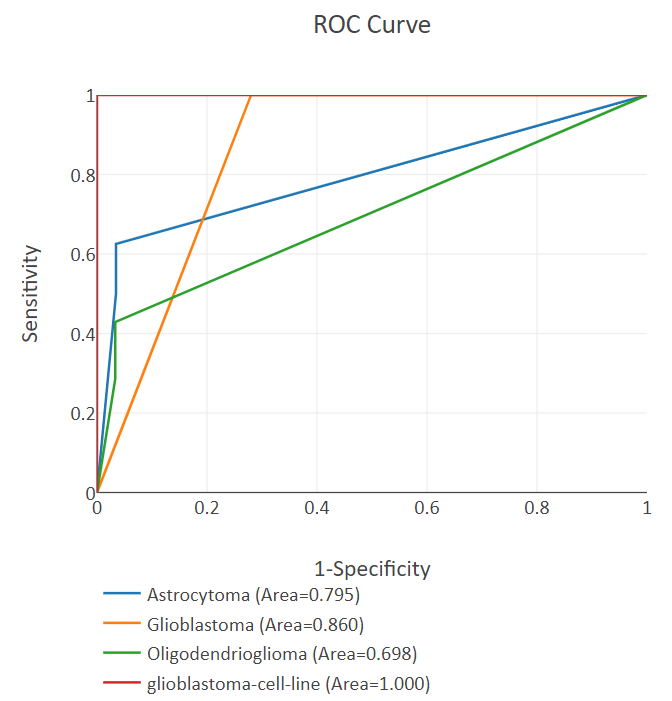
\includegraphics[width=0.4\textwidth]{brain_gse15824_ROC.PNG}}
     \subfloat[Curva A]{
       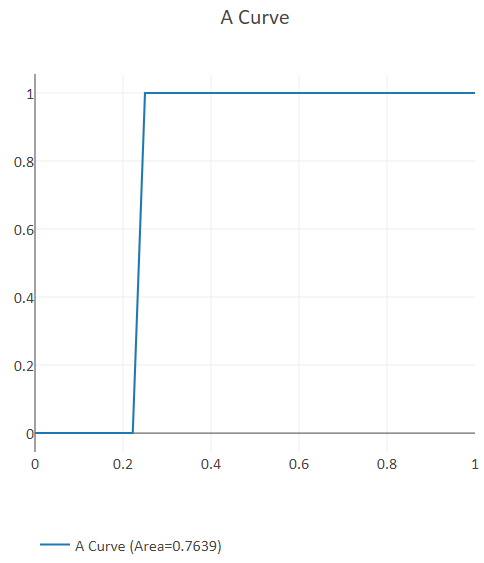
\includegraphics[width=0.4\textwidth]{brain_gse15824_A_CURVE.PNG}}
    \caption{Curvas obtenidas para el fichero brain\_gse15824.csv.}
    \label{fig:10}
\end{figure}

\bigbreak

El fichero de datos brain\_gse15824.csv presenta cuatro clases, los nombres de las clases son Astrocytoma, Glioblastoma, Oligodendrioglioma y Glioblastoma-cell-line. En esta sección se ofrece un análisis e interpretación de los resultados obtenidos al aplicar los métodos de evaluación vistos en secciones anteriores. El análisis e interpretación se realiza de forma independiente para las diferentes clases.

\bigbreak

La exactitud es de $0.757$ unidades, es decir, hay un $75.7$\% de probablidad de acierto en la predicción que realiza el modelo. El área bajo la curva-A es de $0.764$ unidades, un valor notablemente alto. La diferencia entre el área bajo la curva-A y la exactitud es de $0.007$ unidades. 

\bigbreak

La clase Astrocytoma presenta un indicador de sensibilidad bajo, un resultado de $0.5$ indica que tan solo la mitad de los registros de está clase se prediccen de forma correcta. La especificidad es de $0.966$ unidades, esto implica que para intancias en las que la clase es diferente a Astrocytoma, la predicción se hace correctamente el 96.6\% de las veces. El indicador de precisión es de $0.8$ unidades, las instnacias que se predicen de clase Astrocytoma tienen una tasa de acierto del $80$\%. La precisión inversa indica que la predicción es correcta para el 80\% de las instancias que se predicen de una clase diferente a Astrocytoma. El resultado para la precisión inversa es de $0.85$ unidades, la tasa de aciertos en la prediccón de clases diferentes a Astrocytoma es notablemente buena. La razón de verosimilitud positiva presenta un fuerte aumento de la probabilidad de acierto que tiene un registro que se predice de clase Astrocytoma, en concreto supone más de un 45\% de mejora (Tabla \ref{tab:2}). La razón de verosimilitud negativa obtiene un resultado de $0.518$ puntos, esto implica una leve disminución en la probabilidad de que un registro sea de clase Astrocytoma cuando se precdice de una clase diferente, la disminución que presenta es de entorno al 15\% (Tabla \ref{tab:2}). El DOR ofrece un indicador conjunto de las razones de verosimilitud, en general indica una buena capacidad discriminatoria para la clase Astrocytoma. El indice de Youden tiene un valor de $0.46$, un valor poximo a $0.5$ indica una capacidad discriminatoria aceptable para la clase Astrocytoma. El resultado para el coeficiente de correlación de Matthews es de $0.561$ unidades, un valor que indica una fuerte correlación entre clase y predicción (Tabla \ref{tab:3}). El poder disciminante de $0.798$ implica una capacidad discriminatoria postiva para la clase Astrocytoma. El valor de la medida-F implica una tasa aceptable de acierto para instancias en las que la clase o la predicción es Astrocytoma, en este caso la baja sensibilidad obtenida penaliza el resultado obtenido. El markedness es un indicador que agurpa los métodos que miden la exactitud en la predicción, un resultado de $0.675$ implica una notable tasa de acierto. La media geometica y la exactitud balanceada ofrecen un indicador de la tasa de acietos conjunta para instancias de clase Astrocytoma e instancias que no son de clase Astrocytoma, en ambos casos el indicador es notablemente alto. El resultado para la precisión de optimización es de $0.547$ unidades, un valor bajo que se ha visto afectado por la gran diferencia que existe entre sensibilidad y especificidad. El resultado que se obtiene al aplicar Jaccard es de $0.444$ unidades, esto indica un grado de similitud bajo entre clase y predicción.

\bigbreak

La sensibilidad para la clase Glioblastoma es de una unidad, esto implica que todas las instancias de esta clase se clasifican de forma correcta. El indicador de especificidad indica una notable tasa de acierto a la hora de determinar que instancias no pertenecen a la clase Glioblastoma. La precisión de $0.63$ unidades implica una buena tasa de acierto sobre las intancias que se predicen de clase Glioblastoma. La precisión inversa obtiene un resultado de una unidad, la predicción es correcta para todas las instancias que se predicen de una clase diferente a Glioblastoma. La razón de verosimilitud positiva indica un leve aumento (Tabla \ref{tab:2}) en la probabilidad de que una instancia pertenezca a la clase Glioblastoma cuando se predice de esta clase. El indice de Youden indica una capacidad discriminatoria notable para la clase Glioblastoma. El resultado obtenido por el coeficiente de correlación de Matthews es de $0.674$, este valor implica una alta correlación (Tabla \ref{tab:3}) entre la predicción y la clase Glioblastoma. La medida-F indica una tasa notable de acierto en la predicción de la clase. La media geometica y la exactitud balanceada ofrecen indicadores que reflejan una tasa de aciertos notable, ambos métodos agrupan sensibilidad y especificidad. La precisión de optimización indica una buena tasa de acierto para la clase Glioblastoma. El método de Jaccard indica un grado de similitud medio entre la predicción y la clase Glioblastoma.

\bigbreak

d

\bigbreak

La clase Glioblastoma-cell-line muuestra un comportamiento ideal, el modelo es capaz de discriminar entre esta clase y el resto de forma perfecta.

\bigbreak

Los resultados obtenidos para el fichero brain\_gse15824.csv han sido positivos, en general las tasas de acierto han sido notables. Los métodos que se aplicado ayudan a reconocer algunos puntos de mejora, en este caso, la clase Oligodendrioglioma es la que obtiene peores indicadores, el modelo puede mejorarse ajustando la predicción sobre esta clase.

\clearpage

%%%%%%%%%%%%%%%%%%%%%%%%%%%%%%%%%%%%%%%%%%%%%%%%%%%%%%% RESULTADO

\subsubsection{Fichero breast\_gse45827.csv}

\begin{table}[htp]
    \small
    \centering
    \begin{tabularx}{\columnwidth}{Y Y}
        ACC       & AUAC    \\\hline
        $0.914$   & $0.917$ \\\hline
    \end{tabularx}
    \caption{Resultados globales para el fichero breast\_gse45827.csv.}
    \label{tab:12}
\end{table}

\begin{table}[htp]
    \small
    \centering
    \begin{tabularx}{\columnwidth}{l Y Y Y Y Y Y}
                &  Her          & Basal     & Cell\_line & Luminal\_a & Luminal\_b & Normal    \\\hline
        TPR     &  $0.900$      & $0.927$   & $1.000$    & $0.862$    & $0.933$    & $0.857$   \\\hline
        TNR     &  $0.967$      & $0.982$   & $1.000$    & $0.984$    & $0.959$    & $1.000$   \\\hline
        PPV     &  $0.871$      & $0.950$   & $1.000$    & $0.926$    & $0.848$    & $1.000$   \\\hline
        NPV     &  $0.975$      & $0.973$   & $1.000$    & $0.968$    & $0.983$    & $0.993$   \\\hline
        LR+     &  $27.225$     & $50.976$  & -          & $52.586$   & $22.587$   & -         \\\hline
        LR-     &  $0.103$      & $0.075$   & $0.000$    & $0.140$    & $0.070$    & $0.143$   \\\hline
        DOR     &  $263.250$    & $684.000$ & -          & $375.000$  & $324.800$  & -         \\\hline
        YI      &  $0.867$      & $0.909$   & $1.000$    & $0.846$    & $0.892$    & $0.857$   \\\hline
        MCC     &  $0.856$      & $0.916$   & $1.000$    & $0.869$    & $0.861$    & $0.923$   \\\hline
        DP      &  $1.334$      & $1.563$   & -          & $1.419$    & $1.385$    & -         \\\hline
        $F_{1}$ &  $0.885$      & $0.938$   & $1.000$    & $0.893$    & $0.889$    & $0.923$   \\\hline
        MK      &  $0.846$      & $0.923$   & $1.000$    & $0.894$    & $0.832$    & $0.993$   \\\hline
        BCR     &  $0.933$      & $0.954$   & $1.000$    & $0.923$    & $0.946$    & $0.929$   \\\hline
        GM      &  $0.933$      & $0.954$   & $1.000$    & $0.921$    & $0.946$    & $0.926$   \\\hline
        OP      &  $0.918$      & $0.938$   & $1.000$    & $0.894$    & $0.940$    & $0.916$   \\\hline
        Jaccard &  $0.794$      & $0.884$   & $1.000$    & $0.806$    & $0.800$    & $0.857$   \\\hline
    \end{tabularx}
    \caption{Resultados agrupados por clase para el fichero breast\_gse45827.csv.}
    \label{tab:13}
\end{table}

\clearpage

\begin{figure}[htp]
    \centering
     \subfloat[Curva ROC]{
       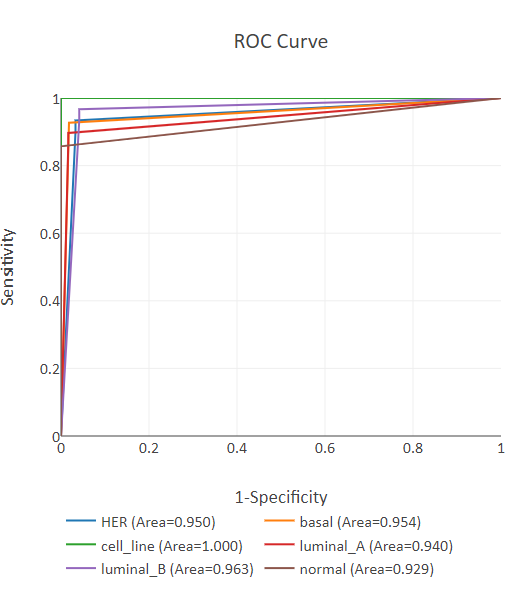
\includegraphics[width=0.4\textwidth]{breast_gse45827_ROC.PNG}}
     \subfloat[Curva A]{
       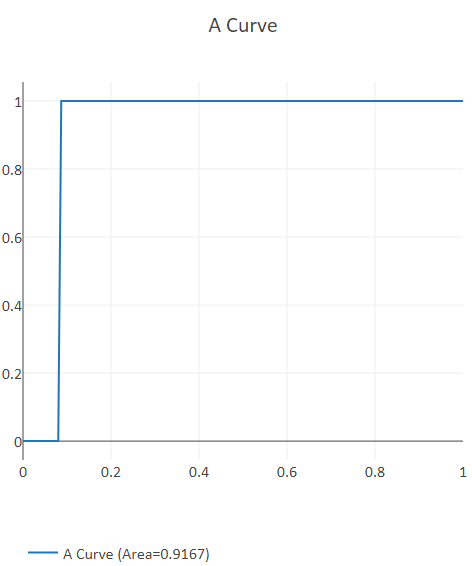
\includegraphics[width=0.4\textwidth]{breast_gse45827_A_CURVE.PNG}}
    \caption{Curvas obtenidas para el fichero breast\_gse45827.csv.}
    \label{fig:11}
\end{figure}

\bigbreak

\lipsum[1]

\clearpage

%%%%%%%%%%%%%%%%%%%%%%%%%%%%%%%%%%%%%%%%%%%%%%%%%%%%%%% RESULTADO

\subsubsection{Fichero colorectal\_gse21510.csv}

\begin{table}[htp]
    \small
    \centering
    \begin{tabularx}{\columnwidth}{Y Y}
        ACC       & AUAC    \\\hline
        $0.980$   & $0.983$ \\\hline
    \end{tabularx}
    \caption{Resultados globales para el fichero colorectal\_gse21510.csv.}
    \label{tab:14}
\end{table}

\begin{table}[htp]
    \small
    \centering
    \begin{tabularx}{\columnwidth}{l Y Y Y}
                &  Normal\_homogenized  & Tumoral\_lcm  & Tumoral\_homogenized  \\\hline
        TPR     &  $0.920$              & $1.000$       & $0.944$               \\\hline
        TNR     &  $1.000$              & $0.930$       & $1.000$               \\\hline
        PPV     &  $1.000$              & $0.972$       & $1.000$               \\\hline
        NPV     &  $0.984$              & $1.000$       & $0.992$               \\\hline
        LR+     &  -                    & $14.333$      & -                     \\\hline
        LR-     &  $0.080$              & $0.000$       & $0.056$               \\\hline
        DOR     &  -                    & -             & -                     \\\hline
        YI      &  $0.920$              & $0.930$       & $0.944$               \\\hline
        MCC     &  $0.951$              & $0.951$       & $0.968$               \\\hline
        DP      &  -                    & -             & -                     \\\hline
        $F_{1}$ &  $0.958$              & $0.986$       & $0.971$               \\\hline
        MK      &  $0.984$              & $0.972$       & $0.992$               \\\hline
        BCR     &  $0.960$              & $0.965$       & $0.972$               \\\hline
        GM      &  $0.959$              & $0.964$       & $0.972$               \\\hline
        OP      &  $0.945$              & $0.943$       & $0.965$               \\\hline
        Jaccard &  $0.920$              & $0.972$       & $0.944$               \\\hline
    \end{tabularx}
    \caption{Resultados agrupados por clase para el fichero colorectal\_gse21510.csv.}
    \label{tab:15}
\end{table}

\clearpage

\begin{figure}[htp]
    \centering
     \subfloat[Curva ROC]{
       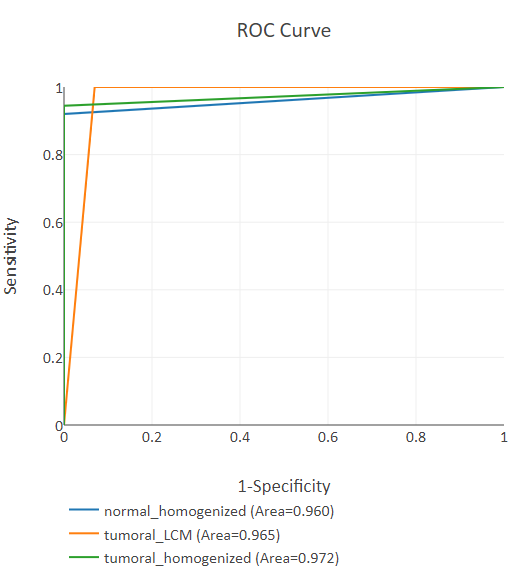
\includegraphics[width=0.4\textwidth]{colorectal_gse21510_ROC.PNG}}
     \subfloat[Curva A]{
       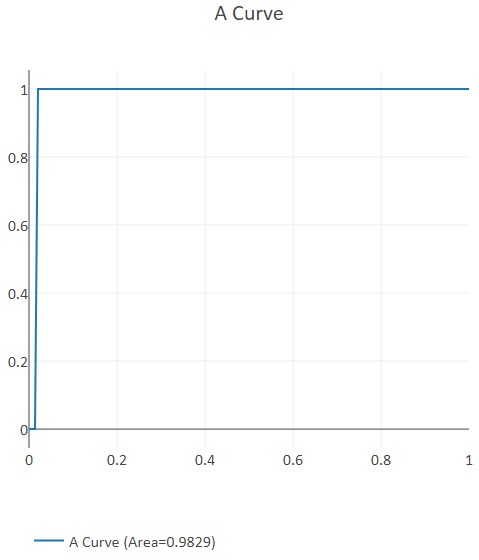
\includegraphics[width=0.4\textwidth]{colorectal_gse21510_A_CURVE.PNG}}
    \caption{Curvas obtenidas para el fichero colorectal\_gse21510.csv.}
    \label{fig:12}
\end{figure}

\bigbreak

\lipsum[1]

\clearpage


%%%%%%%%%%%%%%%%%%%%%%%%%%%%%%%%%%%%%%%%%%%%%%%%%%%%%%% RESULTADO

\subsubsection{Fichero breast\_gse42568.csv}

\begin{table}[htp]
    \small
    \centering
    \begin{tabularx}{\columnwidth}{Y Y}
        ACC       & AUAC    \\\hline
        $0.991$   & $0.996$ \\\hline
    \end{tabularx}
    \caption{Resultados globales para el fichero breast\_gse42568.csv.}
    \label{tab:16}
\end{table}

\begin{table}[htp]
    \small
    \centering
    \begin{tabularx}{\columnwidth}{l Y Y}
                &  Normal               & Tumoral       \\\hline
        TPR     &  $0.933$              & $1.000$       \\\hline
        TNR     &  $1.000$              & $0.933$       \\\hline
        PPV     &  $1.000$              & $0.990$       \\\hline
        NPV     &  $0.990$              & $1.000$       \\\hline
        LR+     &  -                    & $15.000$      \\\hline
        LR-     &  $0.067$              & $0.000$       \\\hline
        DOR     &  -                    & -             \\\hline
        YI      &  $0.933$              & $0.933$       \\\hline
        MCC     &  $0.961$              & $0.961$       \\\hline
        DP      &  -                    & -             \\\hline
        $F_{1}$ &  $0.966$              & $0.995$       \\\hline
        MK      &  $0.990$              & $0.990$       \\\hline
        BCR     &  $0.967$              & $0.967$       \\\hline
        GM      &  $0.966$              & $0.966$       \\\hline
        OP      &  $0.957$              & $0.957$       \\\hline
        Jaccard &  $0.933$              & $0.990$       \\\hline
    \end{tabularx}
    \caption{Resultados agrupados por clase para el fichero breast\_gse42568.csv.}
    \label{tab:17}
\end{table}

\clearpage

\begin{figure}[htp]
    \centering
     \subfloat[Curva ROC]{
       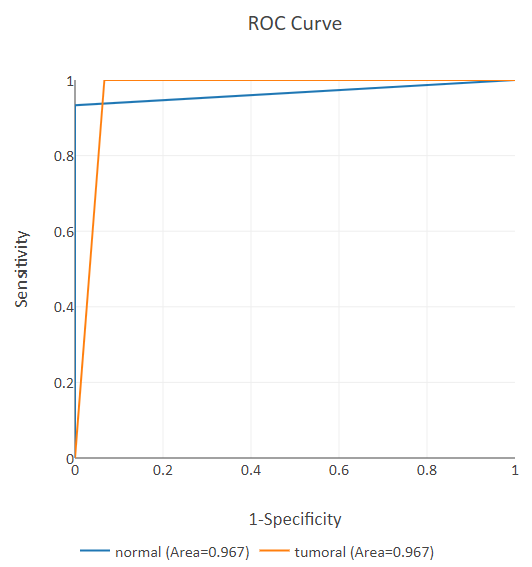
\includegraphics[width=0.4\textwidth]{breast_gse42568_ROC.PNG}}
     \subfloat[Curva A]{
       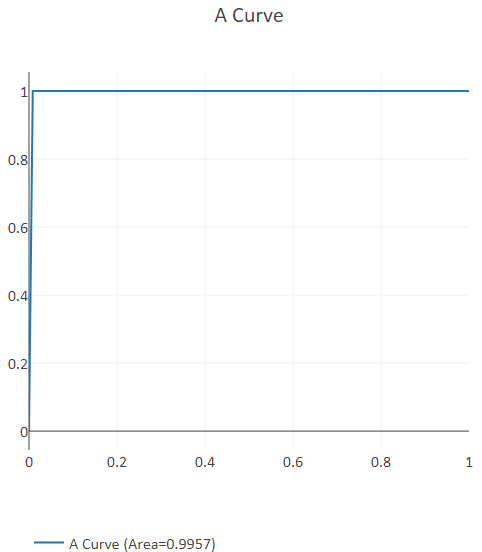
\includegraphics[width=0.4\textwidth]{breast_gse42568_A_CURVE.PNG}}
    \caption{Curvas obtenidas para el fichero breast\_gse42568.csv.}
    \label{fig:13}
\end{figure}

\bigbreak

\lipsum[1]

\clearpage


%%%%%%%%%%%%%%%%%%%%%%%%%%%%%%%%%%%%%%%%%%%%%%%%%%%%%%% RESULTADO

\subsubsection{Fichero gastric\_gse79973.csv}

\begin{table}[htp]
    \small
    \centering
    \begin{tabularx}{\columnwidth}{Y Y}
        ACC       & AUAC    \\\hline
        $0.900$   & $0.921$ \\\hline
    \end{tabularx}
    \caption{Resultados globales para el fichero gastric\_gse79973.csv.}
    \label{tab:18}
\end{table}

\begin{table}[htp]
    \small
    \centering
    \begin{tabularx}{\columnwidth}{l Y Y}
                &  Adenocarcinoma       & Normal        \\\hline
        TPR     &  $0.900$              & $0.900$       \\\hline
        TNR     &  $0.900$              & $0.900$       \\\hline
        PPV     &  $0.900$              & $0.900$       \\\hline
        NPV     &  $0.900$              & $0.900$       \\\hline
        LR+     &  $9.000$              & $9.000$       \\\hline
        LR-     &  $0.111$              & $0.111$       \\\hline
        DOR     &  $81.000$             & $81.000$      \\\hline
        YI      &  $0.800$              & $0.800$       \\\hline
        MCC     &  $0.800$              & $0.800$       \\\hline
        DP      &  $1.052$              & $1.052$       \\\hline
        $F_{1}$ &  $0.900$              & $0.900$       \\\hline
        MK      &  $0.800$              & $0.800$       \\\hline
        BCR     &  $0.900$              & $0.900$       \\\hline
        GM      &  $0.900$              & $0.900$       \\\hline
        OP      &  $0.900$              & $0.900$       \\\hline
        Jaccard &  $0.818$              & $0.818$       \\\hline
    \end{tabularx}
    \caption{Resultados agrupados por clase para el fichero gastric\_gse79973.csv.}
    \label{tab:19}
\end{table}

\bigbreak

\begin{figure}[htp]
    \centering
     \subfloat[Curva ROC]{
       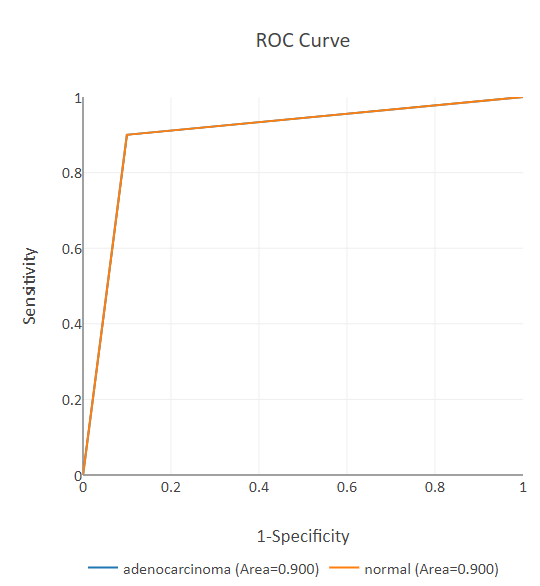
\includegraphics[width=0.4\textwidth]{gastric_gse79973_ROC.PNG}}
     \subfloat[Curva A]{
       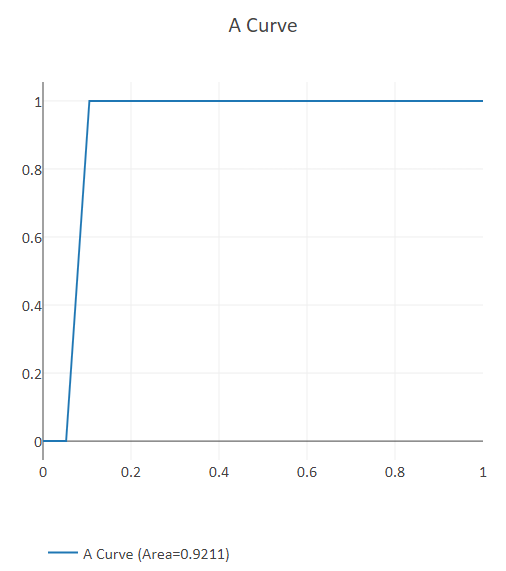
\includegraphics[width=0.4\textwidth]{gastric_gse79973_A_CURVE.PNG}}
    \caption{Curvas obtenidas para el fichero gastric\_gse79973.csv.}
    \label{fig:14}
\end{figure}


La predicción que se realiza a partir de este fichero de datos ofrece unos indicadores de calidad simétricos para ambas clases. La exactitud es de $0.900$ puntos, mientras que el área bajo la curva-A es de $0.921$, esto supone un aumento leve del área bajo la curva en $0.21$ puntos. La sensibilidad, la especificidad, la precisión y la precisión inversa ofrecen el mismo resultado $0.900$, esto indica que los registros de ambas clases, así como, la predicción que se realiza sobre las diferente clases tienen una tasa de acierto del 90\%. EL índice de verosimilitud positiva indica un aumento del 40\% en la probabilidad de que la predicción sea correcta. El índice de verosimilitud negativa indica una disminución del 45\% en la probabilidad de que la predicción se haga de forma incorrecta. El valor de $0.8$ en el indice YI establece una buena capacidad de predicción a partir de la sensibilidad y la especificidad. El coeficiente de correlación de Matthews según la Tabla \ref{tab:3} indica un fuerte grado de correlación entre la clase y la predicción. El DP establece que el modelo presenta una capacidad discriminatoria limitada.

La representación gráfica de la curva ROC ofrece una visión en la que 

\clearpage

%%%%%%%%%%%%%%%%%%%%%%%%%%%%%%%%%%%%%%%%%%%%%%%%%%%%%%% RESULTADO

\subsubsection{Fichero leukemia\_gse14317.csv}

\begin{table}[htp]
    \small
    \centering
    \begin{tabularx}{\columnwidth}{Y Y}
        ACC       & AUAC    \\\hline
        $0.920$   & $0.938$ \\\hline
    \end{tabularx}
    \caption{Resultados globales para el fichero leukemia\_gse14317.csv.}
    \label{tab:20}
\end{table}

\begin{table}[htp]
    \small
    \centering
    \begin{tabularx}{\columnwidth}{l Y Y}
                &  Atl                  & Normal        \\\hline
        TPR     &  $1.000$              & $0.714$       \\\hline
        TNR     &  $0.714$              & $1.000$       \\\hline
        PPV     &  $0.900$              & $1.000$       \\\hline
        NPV     &  $1.000$              & $0.900$       \\\hline
        LR+     &  $3.500$              & -             \\\hline
        LR-     &  $0.000$              & $0.286$       \\\hline
        DOR     &  -                    & -             \\\hline
        YI      &  $0.714$              & $0.714$       \\\hline
        MCC     &  $0.802$              & $0.802$       \\\hline
        DP      &  -                    & -             \\\hline
        $F_{1}$ &  $0.947$              & $0.833$       \\\hline
        MK      &  $0.900$              & $0.900$       \\\hline
        BCR     &  $0.857$              & $0.857$       \\\hline
        GM      &  $0.845$              & $0.845$       \\\hline
        OP      &  $0.753$              & $0.753$       \\\hline
        Jaccard &  $0.900$              & $0.714$       \\\hline
    \end{tabularx}
    \caption{Resultados agrupados por clase para el fichero leukemia\_gse14317.csv.}
    \label{tab:21}
\end{table}

\bigbreak

\begin{figure}[htp]
    \centering
     \subfloat[Curva ROC]{
       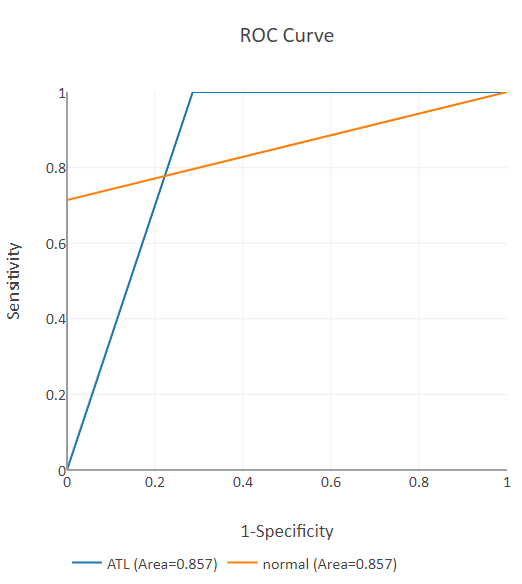
\includegraphics[width=0.4\textwidth]{leukemia_gse14317_ROC.PNG}}
     \subfloat[Curva A]{
       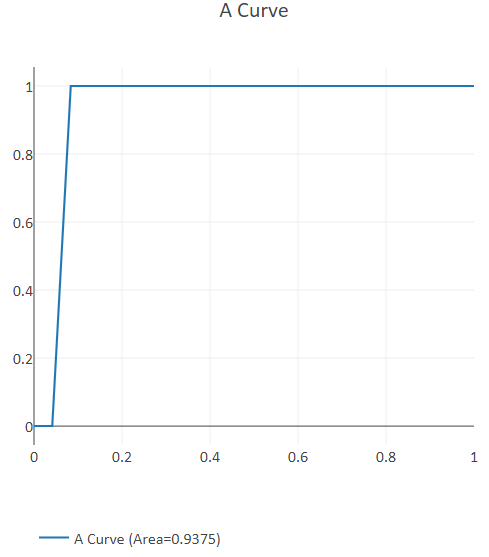
\includegraphics[width=0.4\textwidth]{leukemia_gse14317_A_CURVE.PNG}}
    \caption{Curvas obtenidas para el fichero leukemia\_gse14317.csv.}
    \label{fig:15}
\end{figure}



La exactitud presenta una tasa de aciertos notablemente buena, de cada 100 registros 92 se predicen de forma correcta. El área bajo la curva-A obtiene un valor muy similar al que ha obtenido la exactitud, la diferencia entre ambos métodos supone un aumento en área bajo la curva-A de $0.18$ puntos sobre la exactitud. La sensibilidad y la especificidad representan buenos indicadores, todos los registros de clase Atl se predicen correctamente, los registros de clase Normal tienen un $71.4$\% de probabilidad de acierto. La precisión y la precisión inversa establecen un $90$\% de probabilidad de acierto cuando se predice un registro Atl, por otro la predicción es siempre correcta cuando se predice Normal un registro. El índice de verosimilitud positiva indica un aumento de entorno al 20\% en la probabilidad que tiene un registro que se predice Atl de ser Atl, la clase Normal no presenta índice de verosimilitud positiva debido a que todos los registros que se precicen Normales son efectivamente de clase Normal. El índice de verosimilitud negativa indica que para registros que se predicen de clase Atl hay una reducción del 30\% en la probabilidad de que sea Normal, por otro lado el modelo siempre acierta cuando predice un registro de clase Normal.

\bigbreak

El índice YI presenta un resultado que indica una tasa de aciertos notablemante positiva. El coeficiente de correlación de Matthews de $0.802$ establece una fuerte correlación entre clase y predicción. La medida-F de $0.947$ y $0.833$ implica una que el modelo tiene alta tasa de sensibilidad sobre precisión. El BCR y la GM indican una alta tasa de acierto en la predicción en relación con la sensibilidad y la especificidad del modelo. La precisión de optimización ofrece un resultado en el que se esta penalizando la diferencia entre sensibilidad y especificidad, en valor de $0.714$ en sensibilidad y especificidad implica una reducción leve de la exactitud, sin embargo, a pesar de la penalización sigue ofreciendo un buen nivel de exactitud. El índice de Jaccard establece un nivel de similitud notable entre clase y predicción.

\bigbreak

La representación gráfica que ofrece la curva ROC indican que el modelo ofrece una buena tasa de acierto sobre error en la predicción de ambas clases. La interpretación gráfica de la curva-A establece que la calidad del modelo predictivo es muy positiva.


\clearpage


    \section{Conclusiones}

\subsection{Científicas}

Tras finalizar el conjunto de pruebas, se puede ver más allá de los resultados una mejora en la claridad con la que se presenta la información utilizando la curva-A respecto a la curva ROC. La mejora se hace más notable en modelos con varias clases, a medida que aumenta el número de clases se hace más evidente la mejora. Este aumento de la claridad con la que se presenta la información se puede ver en los resultados obtenidos para el fichero de datos breast\_gse45827.csv, con un total de seis etiquetas se hace complicado interpretar la información que ofrece la curva ROC. La curva-A supone también una alternativa interesante en determinados casos en los que las diferencias entre las distintas curvas ROC es notable. Un nivel de diferencia elevado entre las curvas ROC implica un aumento de la complejidad en la interpretación de la calidad del modelo. En los resultados obtenidos para el fichero bladder\_gse40355.csv, se puede observar que las diferencias que existen entre las tres curvas complican la interpretación de la calidad general del modelo.

\bigbreak

Los resultados obtenidos en la experimentación indican que por norma general el valor del área bajo la curva-A es ligeramente superior al del resto de métodos. La curva-A, en concreto el área bajo la curva-A busca obtener un indicador global de la calidad del modelo, el otro método de carácter global que se ha tratado en este documento es la exactitud. La diferencia entre la exactitud y el área bajo la curva-A es inferior al 2\% para todos los casos prácticos. Este grado de similitud entre ambas medidas aporta una base sólida sobre la que considerar el AUAC como un método fiable a la hora de evaluar la calidad de un modelo predictivo.

\subsection{Académicas}

La evaluación de modelos predictivos es una rama que se enmarca dentro del análisis de datos, esta temática se ha tratado en varias asignaturas. Principalmente es objeto de estudio en minería de datos, en esta asignatura se introduce el uso de Knime como herramienta para el análisis de datos, también se tratan algunos conceptos que se incluyen en este documento como la exactitud, la sensibilidad, la curva ROC, etc. Otras asignaturas como inteligencia artificial o inteligencia de negocio también tratan la temática, aunque de forma más superficial.

\bigbreak

En la actualidad, el aumento en la demanda de servicios informáticos por parte empresas y particulares está provocando un aumento en la cantidad de datos que se están generando. El aumento en la cantidad de datos disponibles, está provocando una tendencia hacia modelos de negocio basados en el análisis y en la explotación de datos. En este sentido, el proyecto ofrece la oportunidad profundizar en las bases de la evaluación de modelos predictivos, una fase clave en muchos procesos de explotación de datos. En el apartado tecnológico, la herramienta Knime ofrece un servicio escalable que es ideal para incorporarlo en proyectos a nivel profesional.

\subsection{Trabajo Futuro}

En este documento se recopilan algunos de los principales métodos que se aplican en la evaluación de modelos predictivos. La propia temática que implica un trabajo de investigación está sujeta a mejoras continuas en la profundidad del estudio que se realiza. A continuación, se enumeran algunos puntos de mejora que se pueden realizar en futuros trabajos.

\begin{itemize}
    \item Profundizar en la comparativa entre la curva-A y la curva ROC.
    \item Profundizar en la comparativa entre el área bajo la curva-A y la exactitud.
    \item Aumentar el número de casos prácticos, ampliando la casuística en los conjuntos de datos.
\end{itemize}

\clearpage


    % BIBLIOGRAFÍA
    \section{Bibliografía}
    \nocite{*}
    \printbibliography[heading=none]

    % ANEXOS
    \section{Anexo I: Preparación del entorno de desarrollo.}

En este anexo se resumen los pasos a seguir para la puesta a punto del entorno de desarrollo, también se incluye la forma de ejecutar el flujo de trabajo y abrir la vista interactiva con el informe de resultados. En primer lugar se tiene que instalar el entorno de desarrollo Knime, la aplicación esta disponible para sistemas operativos Windows, MacOs y Linux. Se puede descargar a través de la siguiente url: \url{https://www.knime.com/downloads}

\bigbreak

Una vez instalado el entorno de desarrollo, se tiene que abrir el fichero EVAL\_MOD\_PRED.knwf incluido en el material. Es posible que en este punto se pida instalar alguna extensión en este caso se recomienda la instalación por defecto que ofrece Knime. Por último, es necesario guardar el flujo de trabajo en una ruta local.

\bigbreak

Para que funcione el proceso automático es importante crear un directorio en la misma ruta donde previamente se ha guardado el flujo de trabajo. El nombre del directorio tiene que ser DATA, hay que tener en cuenta que el nombre ha de ir en mayúsculas. Otro punto importante a la hora de ejecutar el proceso automático, es cambiar el nombre de la clase en la cabecera de los ficheros de datos, por defecto el nombre que se tiene que poner es CLASS. En el nodo CLASS NAMES, se puede modificar el nombre que se usa por defecto para la clase, este nodo situado en el flujo principal. Para finalizar, se tienen que incluir los ficheros en el directorio DATA.

\bigbreak

\begin{figure}[htp]
    \centering
    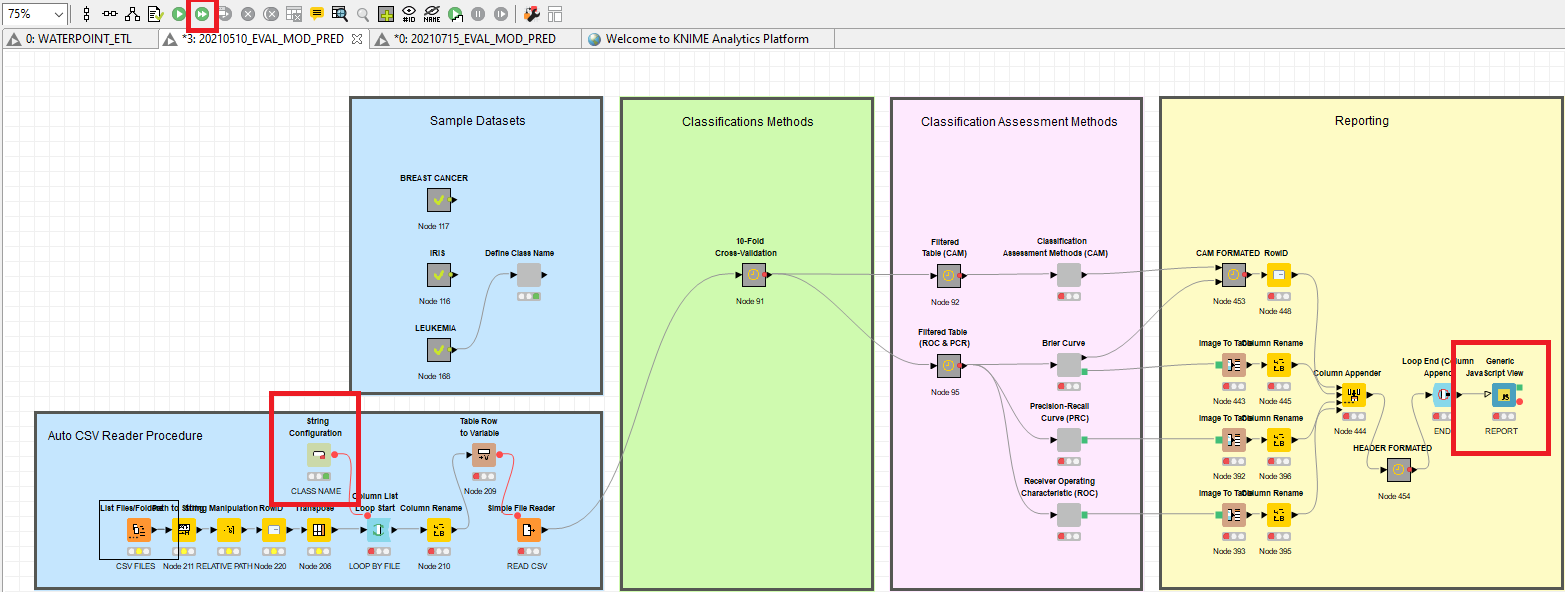
\includegraphics[scale=0.3]{config.png}
    \caption{Flujo principal, se seleccionan en rojo los componentes con los que tiene que interaccionar el usuario.}
    \label{fig:4}
\end{figure}

\bigbreak

Para la ejecución completa del flujo de trabajo, tenemos que hacer clic en el botón verde situado en la barra de herramientas. Alternativamente se puede utilizar el comando shift+F7 para ejecutar el flujo al completo. Los resultados se presentan mediante el nodo REPORT situado en el flujo principal, se puede acceder al informe haciendo clic derecho sobre el nodo y seleccionando la opción de vista interactiva.

\clearpage

\end{document}